\documentclass[22pt, UTF8]{article}
\usepackage{ctex}
\usepackage{graphicx}
\usepackage{multirow}
\usepackage{array}
\usepackage[T1]{fontenc}
\usepackage{mathptmx}
\usepackage{caption}
\usepackage{amsmath, amssymb}
\usepackage{geometry}
\usepackage{fancyhdr}
\usepackage{float}
\usepackage{textcomp}

\geometry{left=3.3cm, right=3.3cm, bottom=3.5cm}
%----------------------------------------------------------------
% 设置页眉和页脚
\pagestyle{fancy}
\lhead{\leftmark} % 页眉的左边显示Section
\rhead{} % 页眉的右边不显示
\renewcommand\headrulewidth{.5pt} % 设置页眉下面的线宽度
\renewcommand\footrulewidth{0pt} % 设置页码上面的线宽度
%-----------------------------------------------------------------
% 设置图片名称的显示格式
\numberwithin{figure}{section}
\captionsetup[figure]{labelfont={bf},name={Fig.},labelsep=period}
% 设置表格名称的显示格式
\numberwithin{table}{section}
\captionsetup[table]{labelfont={bf},name={Tab.},labelsep=period}
%---------------------------------------------------------------
\numberwithin{equation}{section} % 设置公式序号的显示格式

\makeatletter
\@addtoreset{equation}{section}
\makeatother
%---------------------------------------------------------------
\newcommand{\enabstractname}{Abstract} % 设置摘要的显示格式
\newenvironment{enabstract}{
    \par \fontsize{18pt}{0} % “18”是字符串“Abstract”的大小
    \noindent\mbox{}\hfill{\bfseries \enabstractname}\hfill\mbox{}\par
    \vskip 2.5ex}

\linespread{1.5}

\begin{document}
    
\thispagestyle{empty} % 此页不显示页眉、页码等格式
\begin{center}

    \begin{figure}[H]
        \begin{center}
            
\includegraphics[width=4.0cm]{title.eps}
        \end{center}
    \end{figure}

    \vspace{2mm}
    {\LARGE\bf 題目 \par} 
    {\LARGE \textup Text Detection for Natural Scene based on \\MobileNet V2 and U-Net\par}
    \vspace{10mm}
    {\Large 報告者 \par}
    {\LARGE \ 付\ 康为\par}
    \vspace{10mm}
    {\Large 徳島大学大学院\ 先端技術科学教育部 \par}
    {\Large システム創生工学専攻\ 知能情報システム工学コース \par}
    \vspace{10mm}
    %------------------------------------------------------------------
        \begin{figure}[H]
    \begin{center}
        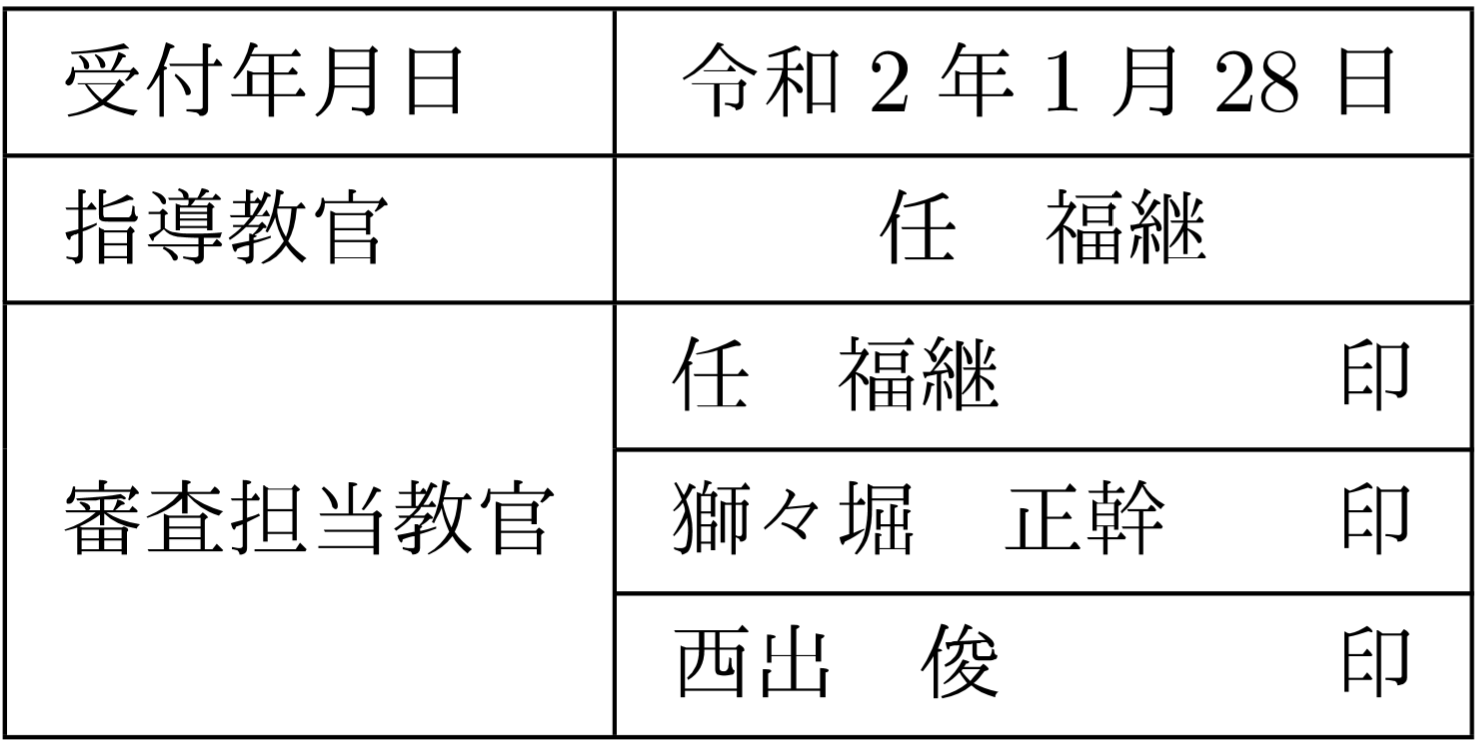
\includegraphics[width=8.0cm]{table.eps}
    \end{center}
\end{figure}
\end{center}

\makeatother

\end{document}